\documentclass[12pt]{article}
\usepackage{epsfig}
\usepackage{graphicx}
\usepackage{color}
\usepackage[frenchb]{babel}
\usepackage{subfigure}
\usepackage{amsmath}
\usepackage{amssymb}
\usepackage{enumerate}

% Pour pouvoir utiliser les accents directement dans LaTeX, sans utiliser les commandes \'
%\usepackage[latin1]{inputenc} % entree 8 bits iso-latin1
\usepackage[utf8]{inputenc} % entree 8 bits utf8, fonctionne avec MikTeX sur Windows.
\usepackage[T1]{fontenc}      % encodage 8 bits des fontes utilisees

% Pour agrandir les marges
\addtolength{\oddsidemargin}{-.875in}
\addtolength{\evensidemargin}{-.875in}
\addtolength{\textwidth}{1.75in}
\addtolength{\topmargin}{-.875in}
\addtolength{\textheight}{1.75in}

\begin{document}
\selectlanguage{french}
\title{Introduction à la robotique mobile : travail pratique 3  \\  Date de remise : 8 décembre 2017, 23h55.}
\author{Instructeur : Philippe Giguère}

\maketitle

\section {Solution par filtre à particules (10 pts)}
Le fichier \textit{src/chariot\_filtre\_particule.py} contient le code de filtre \`a particules.

\begin{figure}[ht]
 \begin{center}
  \begin{tabular}{c}
    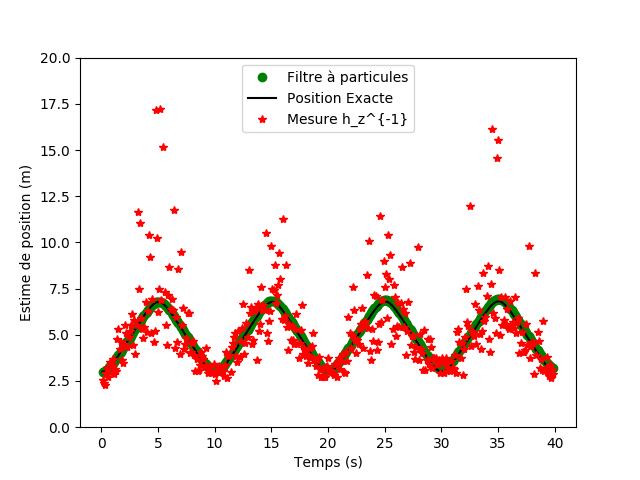
\includegraphics[width=0.75\textwidth]{fig/filtre-particule-chariot.png}
  \end{tabular}
 \end{center}
\vspace{-0.25in}
 \caption{Résultat du filtre à particules sur le chariot}
    \label{chariot-filtre-particule}
\end{figure}

La figure \ref{chariot-filtre-particule} montre le r\'esultat du filtre.

\begin{figure}
\end{figure}

\section{Filtre Kalman étendu (EKF) (40 pts pour GLO-4001, 35 pts pour GLO-7021)}
\label{EKF}

\subsection{Matrices Jacobiennes (10 pts)}

\subsubsection{Détermination de $\Gamma$}
Soit nous définissons $\Gamma$ comme la matrice de dérivé des fonctions de mesure selon la commande:
\begin{equation}
\Gamma =
\begin{bmatrix}
    0   \\
    \\
    \dfrac{e^{u/2}}{(1+e^{u/2})^2} \\
\end{bmatrix}
\end{equation}

\subsubsection{Détermination de $\Lambda$}
\begin{equation}
\Lambda =
\begin{bmatrix}
    \dfrac{-0.07}{d^2} & 0
\end{bmatrix}
\end{equation}

\subsection{Implémentation du filtre EKF (30 pts pour GLO-4001, 25 pts pour GLO-7021)}

Le fichier \textit{src/kalman.py} contient le code de filtre de Kalman étendu.

\subsubsection{Vous connaissez exactement la position initiale du robot au départ.}

\begin{figure}[ht]
 \begin{center}
  \begin{tabular}{c}
    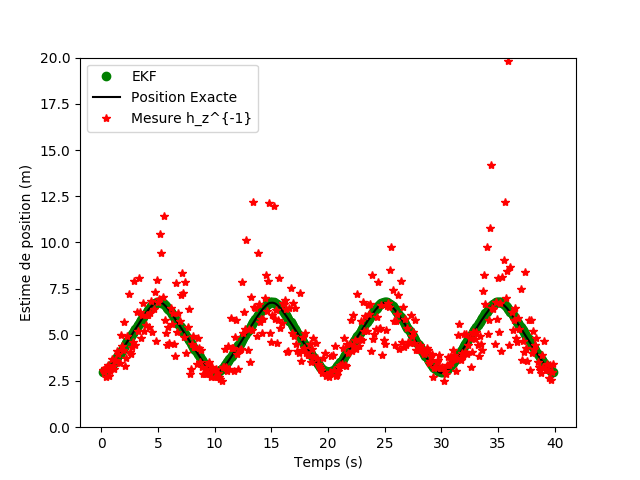
\includegraphics[width=0.75\textwidth]{fig/kalman-position-exacte.png}
  \end{tabular}
 \end{center}
\vspace{-0.25in}
 \caption{Résultat du filtre de Kalman lorsque la position de départ est exacte}
    \label{kalman-position-exacte}
\end{figure}

\subsubsection{Vous avez une bonne idée de la position initiale du robot au départ, mais vous n'êtes pas confiant à $100~\%$.}

\begin{figure}[ht]
 \begin{center}
  \begin{tabular}{c}
    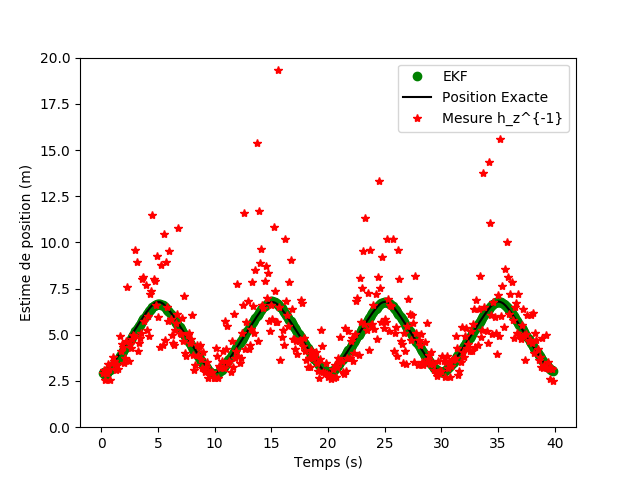
\includegraphics[width=0.75\textwidth]{fig/kalman-position-exacte-incertitude.png}
  \end{tabular}
 \end{center}
\vspace{-0.25in}
    \caption{Résultat du filtre de Kalman lorsque la position de départ est exacte, mais avec une incertitude.}
    \label{kalman-position-exacte-incertitude}
\end{figure}

\subsubsection{Vous croyez connaitre exactement la position initiale du robot au départ, mais cette valeur est, dans les faits, erronée.}

Deux cas peuvent se produire:
\begin{enumerate}
    \item On ne fait pas de corrections
    \item On fait une correction
\end{enumerate}

\begin{figure}[ht]
 \begin{center}
  \begin{tabular}{c}
    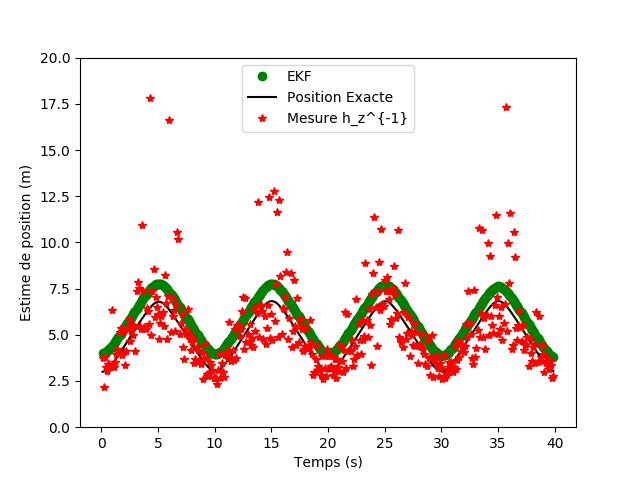
\includegraphics[width=0.75\textwidth]{fig/kalman-position-err-certitude-pas-correction.png}
  \end{tabular}
 \end{center}
\vspace{-0.25in}
    \caption{Résultat du filtre de Kalman lorsque la position de départ est considérée comme exacte, mais est fausse (sans la correction)}
    \label{kalman-position-err-certitude-pas-correction}
\end{figure}

\begin{figure}[ht]
 \begin{center}
  \begin{tabular}{c}
    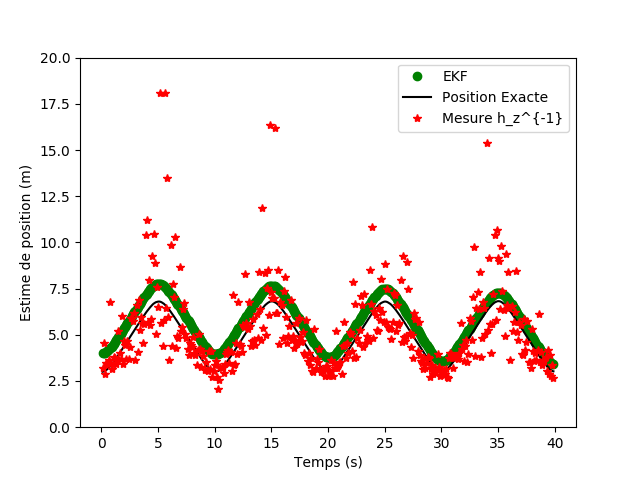
\includegraphics[width=0.75\textwidth]{fig/kalman-position-err-certitude-correction.png}
  \end{tabular}
 \end{center}
\vspace{-0.25in}
    \caption{Résultat du filtre de Kalman lorsque la position de départ est considérée comme exacte, mais est fausse (avec la correction)}
    \label{kalman-position-err-certitude-pas-correction}
\end{figure}

\subsubsection{Vous n'êtes pas sûr que $d=d_{init}+1$ est la bonne position de départ du chariot.}

\begin{figure}[ht]
 \begin{center}
  \begin{tabular}{c}
    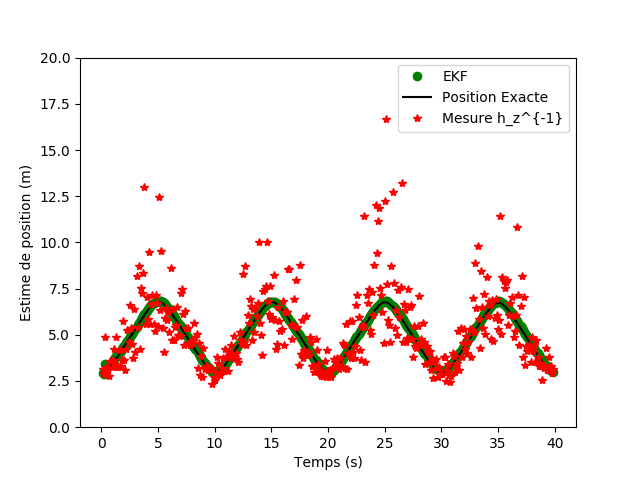
\includegraphics[width=0.75\textwidth]{fig/kalman-position-err-incertitude.png}
  \end{tabular}
 \end{center}
\vspace{-0.25in}
    \caption{Résultat du filtre de Kalman lorsque la position de départ est fausse, mais avec une incertitude.}
    \label{kalman-position-err-incertitude}
\end{figure}


\section {Localisation globale par filtre à particules (35 pts)}

\subsection{Cas 1 : l'angle est connu (GLO-4001 : 30 pts, GLO-7021 : 20 pts)}

\begin{itemize}
\item une justification de votre choix $\sigma_{angle}$;
\item les divers paramètres utilisés dans le filtre;
\item description qualitative de la distribution des particules au fil du temps.
\end{itemize}

\end{document}
